\usetikzlibrary{shapes,snakes}

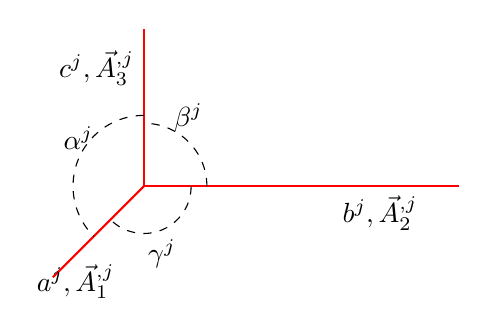
\begin{tikzpicture}
\coordinate (O) at (0,0,0);
\coordinate (A) at (4,0,0);
\coordinate (B) at (0,2,0);
\coordinate (C) at (0,0,3);
\draw[thick,red] (O) -- (A);
\draw[thick,red] (O) -- (B);
\draw[thick,red] (O) -- (C);
\path (O)+(0,0,0) -- (A)+(0,0,0) node [near end, below] {$b^j,  \vec{A}^{,j}_2$};
\path (O)+(0,0,0) -- (B)+(0,0,0) node [near end, left] {$c^j,  \vec{A}^{,j}_3$};
\path (O)+(0,0,0) -- (C)+(0,0,0) node [near end, below] {$a^j,  \vec{A}^{,j}_1$};
\draw[dashed,-](0.6,0,0) arc(0:-135:0.6) node[midway,below]{$\gamma^j$};
\draw[dashed,-](0.8,0,0) arc(0:90:0.8) node[midway,above]{$\beta^j$};
\draw[dashed,-](0,0.9,0) arc(90:225:0.9) node[midway,above]{$\alpha^j$};
%\draw[thick,-] (A) arc - (B);
%\draw[dashed] (\rvec,0,0) arc (0:90:\rvec);
%\draw[thick,->] (0,0,0) --  (2,0,0) node[anchor=north east]{$a$}(aVec);
%\draw[thick,->] (0,0,0) -- (0,2,0) node[anchor=north west]{$b$}(bVec);
%\draw[thick,->] (0,0,0) -- (0,0,2) node[anchor=south]{$c$}(cVec);
\end{tikzpicture}
